\chapter{Background}

\section{Machine Learning}

 Machine learning is a method of analyzing data in which a 
computer automatically iterates through large amounts of data 
without explicit programming to find patterns hidden in the data. 
The purpose of machine learning is to improve computer performance 
on a specific task over time through learning from data.
In other words, machine learning allows computers to adapt 
and improve performance on their own. 
Machine learning algorithms can be classified into two main 
categories: supervised learning and unsupervised learning. 

In supervised learning, a model is trained on a labeled dataset,
which consists of input and corresponding output data. The model 
learns a function which maps the input data to the output data.
Once the model has learned this function, it can be used to make
predictions on unseen data, also known as out-of-sample data, 
that was not part of the original training dataset.
As an example, consider the task of predicting survival on the 
Titanic: the "Titanic - Machine Learning from Disaster" 
competition hosted by Kaggle \cite{titanic} requires participants 
to develop a model that accurately predicts whether an each person
on board survived the Titanic disaster or not. 
The model should be developed using the data in the training set.
The training set consists of information such as the gender and 
passenger ship class of each passenger on board and the results of 
whether the passenger survived or not.
The training set includes information about each passenger, such 
as their gender, age and ship class, and the outcome of whether 
they survived or not. This labeled data is used to build a machine
learning model that can predict whether they survived based on 
other available information of the passengers.

In contrast to supervised learning models, which rely on labeled 
training data, unsupervised learning models do not use such data.
Since the goal of unsupervised learning is to find unknown patterns
that exist in the data, we only provide the input data to the model.
The model discovers regularities and features on its own, without
the guidance of labeled training data.

\begin{figure}[h]
  \centering
  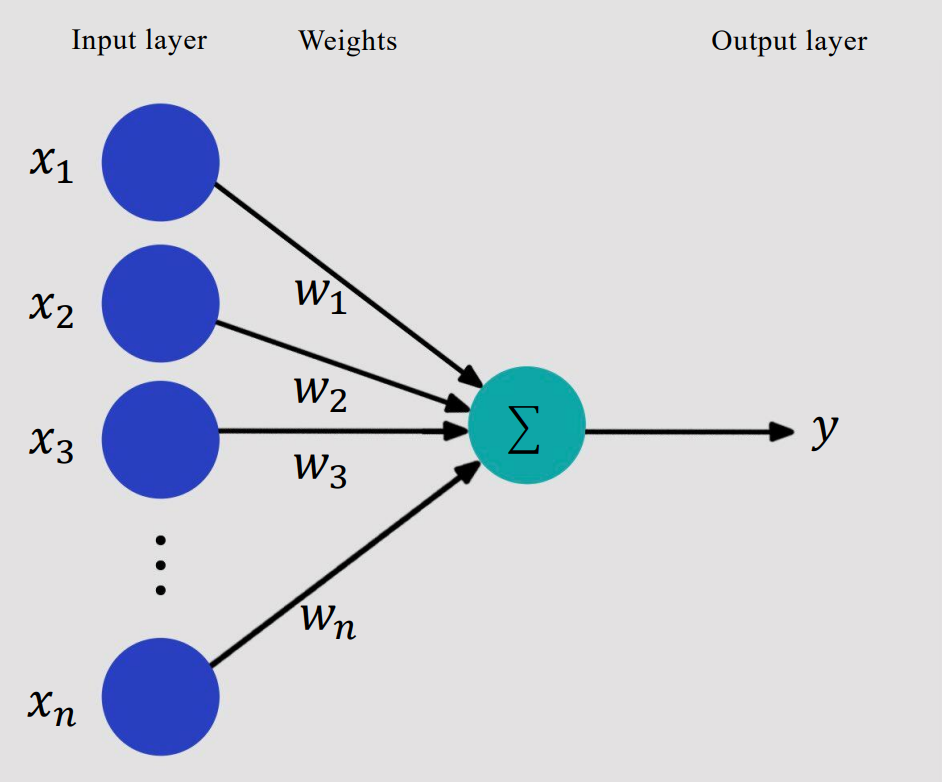
\includegraphics[width=100truemm]{resources/2_background/simple_perceptron.pdf}
  \caption{
    An example of simple perceptron.
  }
  \label{simple_perceptron}
\end{figure}

\section{Neural Networks}
 Neural networks are a kind of machine learning algorithms which 
algorithm is modeled after the function and structure of human 
neural circuits and consist of a large number of interconnected 
processing nodes called neurons.
Frank Rosenblatt's simple perceptron \cite{Rosenblatt1958ThePA} was 
an early example of an artificial neural network. 
Simple perceptron consists of a single neuron that receives inputs 
from multiple sources and generates a single output. 
The structure of it is shown in Figure \ref{simple_perceptron}. 
The figure clearly shows how the perceptron processes received inputs.
The inputs $x_1, x_2 ... x_n$ are multiplied by their respective weights
$w_1, w_2 ... w_n$ and summed to produce the output $y$.
This can be expressed mathematically as follows:
\begin{equation}
  \label{perceptron_output}
  y = \sum_{k}w_k x_k + b
\end{equation}
where $b$ is a term called bias which is a variable that determines 
whether or not the output $y$ is set to 1.
During simple perceptron training, the goal is to find the optimal 
weights $w_1, w_2 ... w_n$, that will produce the correct output for 
a given set of inputs.
However, simple perceptrons are limited in its learning ability because 
they can only model linear relationships between inputs and outputs.
Therefore more complex neural networks are needed for learning tasks 
that require the modeling of nonlinear relationships.
A multilayer perceptron, which is a multilayer version of a simple 
perceptron, is one example. Figure \ref{multilayer_perceptron} shows
the most basic multilayer perceptron, which consists of three layers: 
an input layer, a hidden layer, and an output layer.

\begin{figure}[h]
  \centering
  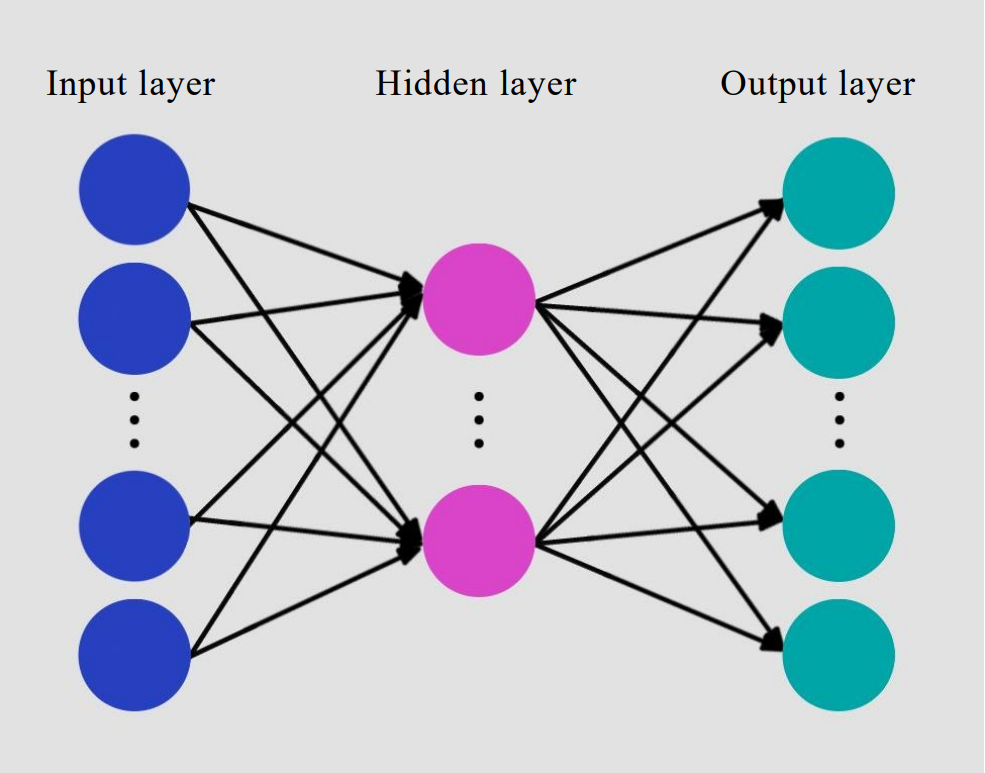
\includegraphics[width=100truemm]{resources/2_background/multi_layer_perceptron.pdf}
  \caption{
    An example of multilayer perceptron.
  }
  \label{multilayer_perceptron}
\end{figure}
While Figure \ref{simple_perceptron} consists of an input layer and an 
output layer, Figure \ref{multilayer_perceptron} has an additional hidden 
layer. The addition of this hidden layer let the network capture nonlinear
relationships between input data and output data.
In Figure \ref{multilayer_perceptron}, there is only one hidden layer,
but it is possible to have multiple hidden layers in a multi-layer perceptron.
In this type of neural network, the data flows in only one direction, without 
looping back or branching off. The models which have this structure is known
as a Feed-forward Neural Networks (FNNs), 
and the structure is a key characteristic of multi-layer perceptrons.
In this paper, we are utilizing FNNs.

\section{Deep Neural Networks}
 There is an area of neural networks called deep learning. 
It used Deep Neural Networks (DNNs), which are characterized by their structure
of having three or more layers, including one or more hidden layers, as models \cite{8114708}.
As previously mentioned, the addition of a hidden layer to a simple perceptron 
enables the creation of a multilayer perceptron, which is capable of learning 
nonlinear relationships. 
Intuitively, it makes sense that a multilayer perceptron with additional 
hidden layers would be able to represent more complex relationships.
This is the concept behind DNNs, which get their name from the fact that they 
have multiple \textit{deep} layers of neurons.
Since DNNs are also a kind of a machine learning algorithm, the goal of learning
for the network is determining the best values of the weights and biases. 
Running the program with the learned weights is called \textit{inference}.

Deep learning has been successfully applied in many such as medical department \cite{medical}, 
self-driving \cite{do2018real}, translation \cite{translation}, art \cite{zou2020stylized},
interior design \cite{interior}, and more.
As we mentioned before, the basic form of deep neural network is a neural network with 
multiple hidden layers, but in the fields addressing image and time series data,
specialized neural network architectures are utilized to better suit the 
characteristics of those types of data.

\section{Convolutional Neural Networks}
 Convolutional Neural Network (CNN) is one of the deep learning architectures. 
CNNs are very effective for tasks processing data with a grid-like structure, 
such as images.

Before describing the structure of CNNs, let us explain how computers represent 
and process image data. A digital image is composed of a grid of small elements 
called pixels, each of which represents the intensity of light and color at 
that location in the image.
In color images, these values are represented by three channels: 
red, green, and blue. Each pixel is assigned a numerical value 
between 0 and 255 for each channel, as shown in Figure \ref{structure-of-image}.
CNNs are designed to process this grid-like structure.

\begin{figure}[h]
  \centering
  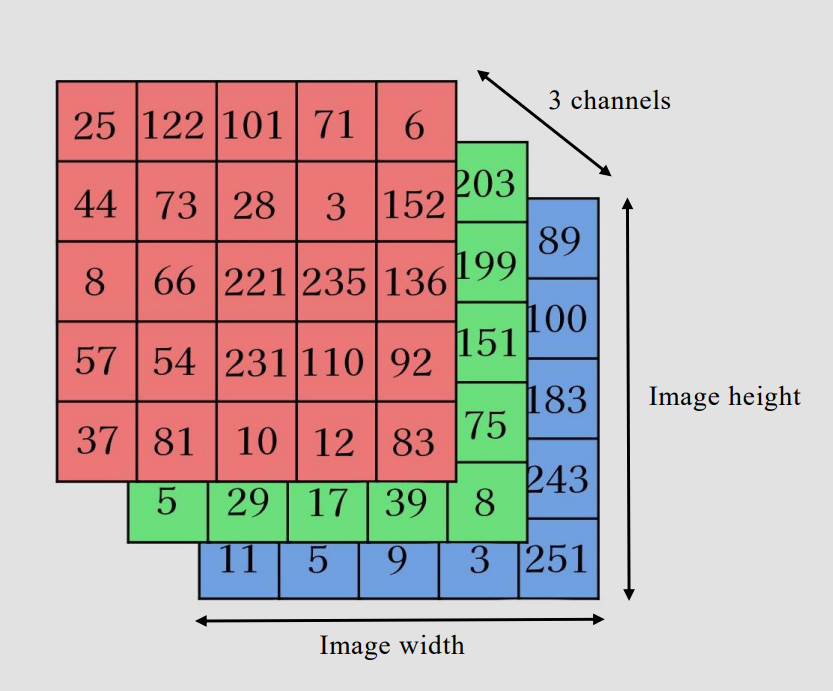
\includegraphics[width=90truemm]{resources/2_background/imagedata.png}
  \caption{
    Structure of a color image.
  }
  \label{structure-of-image}
\end{figure}


\begin{figure}[b]
  \centering
  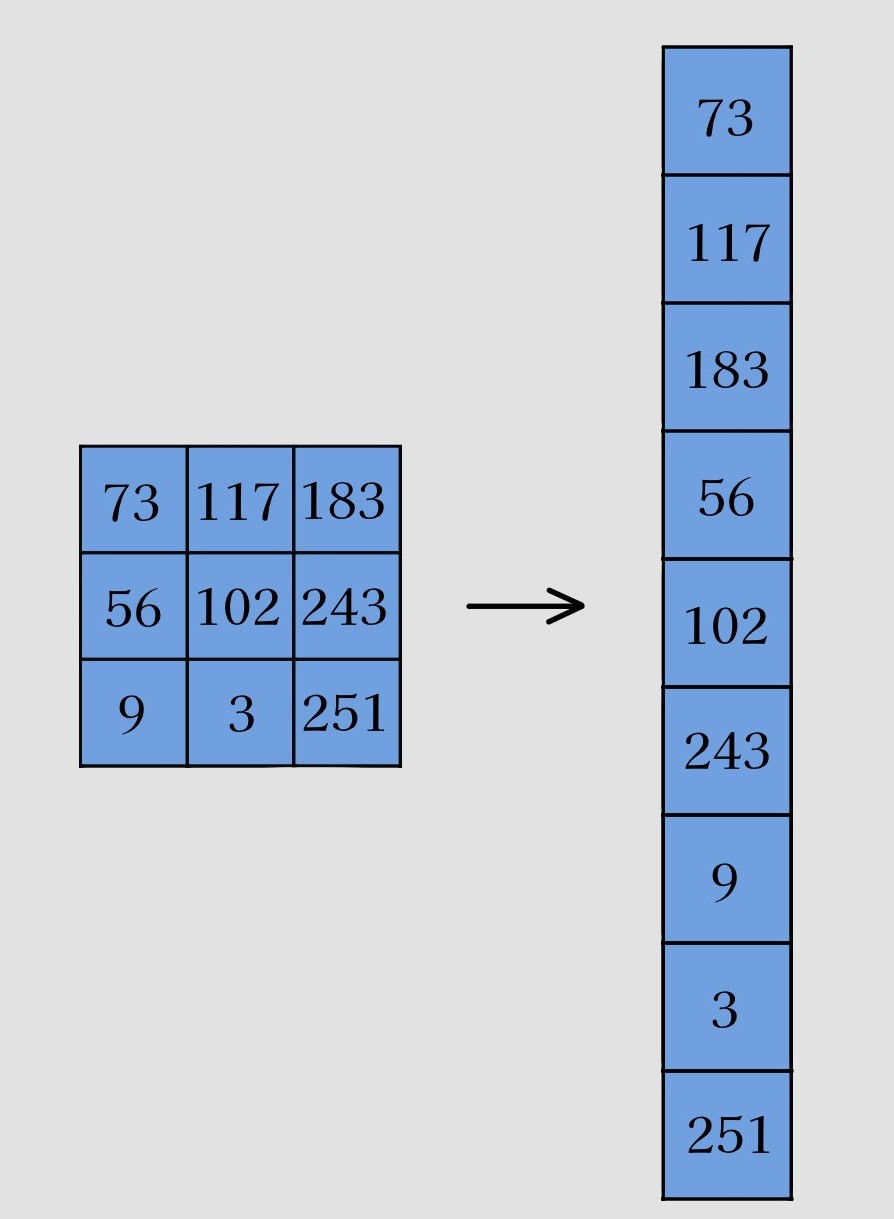
\includegraphics[width=70truemm]{resources/2_background/dimension.png}
  \caption{
    Converting 3x3 matrix data into a 9x1 vector.
  }
  \label{converting-imageddata}
\end{figure}
\clearpage
As previously mentioned, CNNs were developed specifically to process image data.
While it is possible to use traditional neural networks, such as FNNs,
for this purpose, the input must be arranged as a single vertical row, as depicted
in Figure \ref{converting-imageddata}. 
Although vertical and horizontal positional information is important for an image,
with this approach, the vertical and horizontal positions of the pixels are lost 
when the image is transformed into a one-dimensional format. It is optimal to 
treat images as two-dimensional data, and this is possible using CNNs.

CNNs are comprised of three types of layers:
convolutional layers, pooling layers, and fully-connected layers.
As the input image passes through the convolutional, pooling, and fully-connected
layers as shown in Figure \ref{example-of-CNN}, its features are transformed and combined, resulting 
in a set of class scores that can be used for tasks such as classification and 
regression. 

\begin{figure}[h]
  \centering
  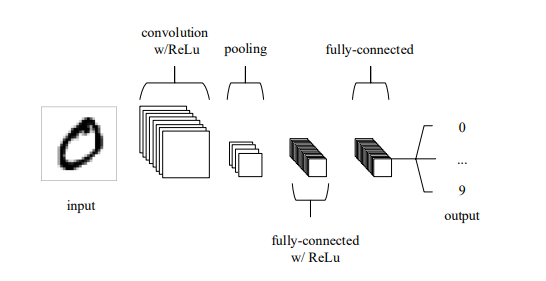
\includegraphics[width=120truemm]{resources/2_background/ex-CNN.pdf}
  \caption{
    An example of CNNs architecture,
    taken from \cite{o2015introduction}.
  }
  \label{example-of-CNN}
\end{figure}
Figure \ref{example-of-CNN} is for giving a rough understanding of the overall 
CNNs architecture.
The architecture in the image is for MNIST \cite{deng2012mnist} classification, 
or to determine whether the input image corresponds to any of the categories 
0 to 9. A detailed explanations of the individual layers will follow.

The convolution layer performs operations to extract features from images using 
a filter known as a kernel.
The kernel typically takes a size much smaller than the input image. 
As shown in Figure \ref{convolution-process}, the convolution operation involves calculating the 
element-wise product of the kernel and the input tensor at each position of 
the tensor and summing the results to obtain the output value. 
The output values obtained from calculating the convolution operation on the 
entire input image will be tensor known as a feature map.
The feature map, as the name implies, is a characteristic quantity 
extracted by the kernel. By repeating the convolution operation using multiple
kernels, multiple feature maps representing various features of the input 
image can be generated. 
The size of the feature map can be controlled by changing the size of the kernel and the number 
of pixels by which the kernel is shifted, known as the stride. 
(The stride in Figure \ref{convolution-process} is 1.)
A larger kernel size or stride will result in a smaller feature map, 
while a smaller kernel size or stride will result in a larger feature map.


The pooling layer is used to reduce the size of the feature maps produced by 
the convolutional layer, the process of which is called down-sampling. 
One of the most commonly used pooling methods is max pooling.
In max pooling, the output of the pooling layer is the maximum value of 
the smallest region of the input feature map. 
The small region is typically a square window with a fixed size, and the maximum
value within this window is taken as the output for the pooling layer at that position.
The example of this process is as shown in Figure \ref{max-pooling}.
Besides max pooling, there is mean pooling, which takes the average of 
a small region of the input feature map. 
Pooling process reduces the size of the feature map and the number of parameters 
in the model, which helps to reduce overfitting.
\vspace{1.2cm}
\begin{figure}[h]
  \centering
  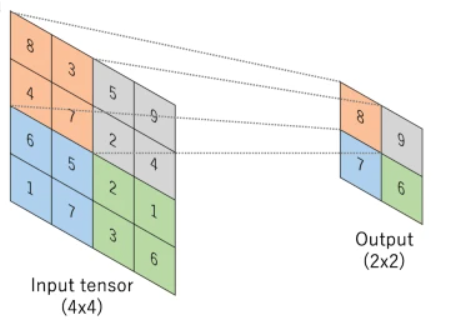
\includegraphics[width=100truemm]{resources/2_background/max_pooling.pdf}
  \caption{
    An example of max pooling,
    taken from \cite{yamashita2018convolutional}.
  }
  \label{max-pooling}
\end{figure}

\begin{figure}[p]
  \centering
  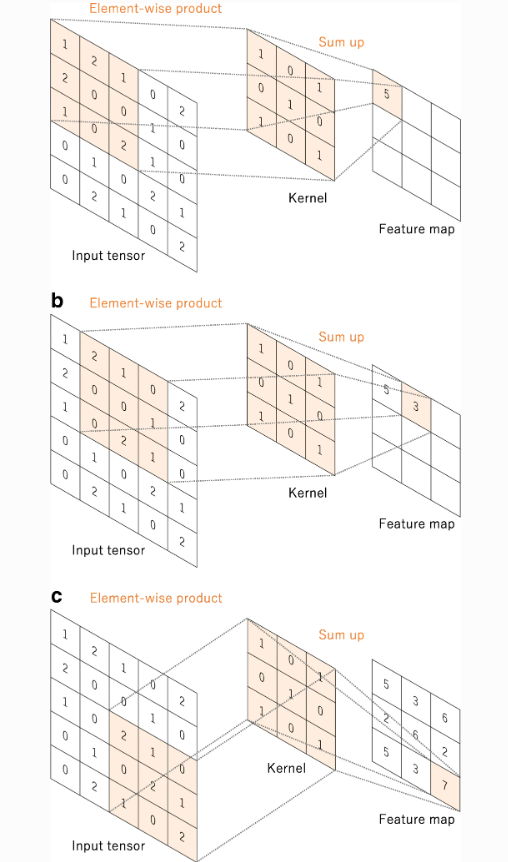
\includegraphics[width=90truemm]{resources/2_background/ex-convolution.pdf}
  \caption{
    Examples of convolution operation,
    taken from \cite{yamashita2018convolutional}.
  }
  \label{convolution-process}
\end{figure}
\clearpage

The fully-connected layer has structures each neuron of which is connected 
to every neuron in the previous layer. This allows for the combination of 
the feature maps generated by the previous layers, resulting in a 
one-dimensional output.  

\section{Transformers}
 Transformers were first introduced by Vaswani \textit{et al}. \cite{vaswani2017attention}
It is a neural network that learns context, and hence meaning, by tracking the
relationships between successive sets of data, and is used primarily in the 
field of natural language processing. 
It uses a self-attention mechanism without any convolutional neural networks 
or recurrent neural networks, which allows parallel computation and greatly 
contributes to shortening the learning rate.
It is characterized by the fact that it is not necessary to process time-series 
data sequentially. This means that, for example, when the input data is a 
natural language sentences, it is not necessary to process the data by starting 
at the beginning of the sentences and working towards the end.

While the Transformer architecture is mainly known for its applications in 
natural language processing, DETR \cite{DBLP:journals/corr/abs-2005-12872} employs 
this technique in the context of object detection model. The reason for this is that 
Transformers can make accurate predictions without the need for additional, complex 
post-processing steps. In this paper we also use Transformers in our stroke prediction 
model.
